\chapter{Introduction}\label{chapter:introduction}

Introductory programming classes are big and hard to teach. Programming classes on some college campuses are reaching hundreds or thousands of students~\cite{biggestClass}. Massive Open Online Courses (MOOCs) on programming have drawn tens or hundreds of thousands of students~\cite{codewebs}. Millions of students complete programming problems online through sites like Khan Academy.

Massive classes generate massive datasets of solutions to the same programming problem. The problem could be exponentiating a number, computing a derivative, or transforming a string in a specific way. The solutions are typically a single function that prints or returns an answer. A terse solution might contain a couple of lines. An excessively verbose solution might contain over twenty lines.

This thesis revolves around clustering and visualizing massive datasets of solutions in novel, human-readable ways. For example, rather than representing solutions as points in a projection of a high-dimensional space into two or three dimensions, OverCode's deterministic unsupervised clustering pipeline synthesizes platonic solutions that each represent entire stacks of solutions. For example, the solution shown in Figure~\ref{largestStack} represents 1538 solutions~\cite{overcode}. OverCode is the first of several systems for clustering and visualizing solutions and solution variation that were developed in this thesis.

\begin{figure}
\centering
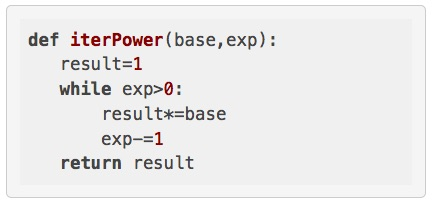
\includegraphics[width=0.5\linewidth]{Body/figures/overcode/largest_stack_cropped.jpg}
\caption{A solution synthesized by OverCode that represents 1538 student solutions.}
\label{largestStack}
\end{figure}

\section{Solution Variation}

The taxonomy for {\it solution variation} used in this thesis has three branches: correctness, approach, and readability. Since correctness is difficult to prove for an arbitrary piece of code, it is approximated in industry and education by correctness with respect to a set of test cases. In education, the machinery that checks for correctness is often called an autograder.

There is a wide range of solutions that pass all the test cases and are labeled correct by the autograder, but they are not all equally good. Figure~\ref{table:diffapproaches} shows three different solutions of widely varying approach and readability that are correct with respect to the autograder test cases.

\begin{figure}
\begin{tabular}{ll}
{\bf Iterative Solution} & {\bf Recursive Solution} \\
\begin{minipage}{0.5\linewidth}
\begin{lstlisting}[basicstyle=\linespread{1.0}\ttfamily\footnotesize,language=python]
def power(base,exp):
    result=1
    while exp>0:
        result*=base
        exp-=1
    return result
\end{lstlisting}
\end{minipage}
&
\begin{minipage}{0.5\linewidth}
\begin{lstlisting}[basicstyle=\linespread{1.0}\ttfamily\footnotesize,language=python]
def power(base,exp):
    if exp == 0:
        return 1
    else:
        return base * power(base, exp-1)
\end{lstlisting}
\end{minipage} \\
% \end{tabular}

% \begin{tabular}{l}
{\bf Poorly Written Solution} & \\
\begin{minipage}{0.5\linewidth}
\begin{lstlisting}[basicstyle=\linespread{1.0}\ttfamily\footnotesize,language=python]
def power(base, exp):
    tempBase=base
    result = base

    if type(base)==int:
        while exp==0:
            result = 1
            print(result)
            break
        exp=exp-1
        while exp >0:
            tempCal=abs(tempBase)
            exp=exp-1
            while exp<0:
                break
            for i in range (1,tempCal):
                result=result+base
                tempCal=tempCal-1
                tempRes=base
            base=result
        return(result)

    else:
        result = 1
        while exp > 0:
            result = result* base
            exp = exp- 1
        return result
\end{lstlisting}
\end{minipage} 
\end{tabular}
\caption{Three different solutions that exponentiate a base to an exponent. They are all marked correct by the autograder because they pass all the autograder test cases.}
\label{table:diffapproaches}
\end{figure}

Solutions can have different approaches. For example, a student might be subversive and disregard a request by the teacher to solve the problem without using an existing equivalent library function. Or the student might include unnecessary lines of code that reveal possible misconceptions about how the language works. Figure~\ref{table:morediffapproaches} gives an example of each.

\begin{figure}
\begin{tabular}{ll}
{\bf Subversive Solution} &  \\
\begin{minipage}{0.5\linewidth}
\begin{lstlisting}[basicstyle=\linespread{1.0}\ttfamily\footnotesize,language=python]
def power(base, exp):
  return base**exp
\end{lstlisting}
\end{minipage}
& \\
% \end{tabular}

% \begin{tabular}{l}
{\bf Solution with Unnecessary Statement} & \\
\begin{minipage}{1.0\linewidth}
\begin{lstlisting}[basicstyle=\linespread{1.0}\ttfamily\footnotesize,language=python]
def power(base,exp):
 result=1
 while exp>0:
     result=result*base
     exp-=1
     continue #keyword here does not change execution
 return result
\end{lstlisting}
\end{minipage} 
\end{tabular}
\caption{Two different approaches to solving the problem. The first disregards teacher instructions to not use equivalent library functions and the second includes the keyword \texttt{continue} in a place where it is completely unnecessary, casting doubt on student understanding of the keyword \texttt{while}.}
\label{table:morediffapproaches}
\end{figure}

Approaches can be common or uncommon. One can think of the students submitting solutions as a generative function that produces a distribution of solutions we could characterize and take into account while teaching or designing new course material. Figure~\ref{table:commonuncommon} shows the most common and one of the most uncommon solutions produced by students for a problem assigned in 6.00x, an introductory programming course offered on edX in the fall of 2012. Uncommon solutions may be highly innovative or extraordinarily poor.

\begin{figure}
\begin{tabular}{ll}
{\bf Common Solution} & {\bf Uncommon solution} \\
\begin{minipage}{0.5\linewidth}
\begin{lstlisting}[basicstyle=\linespread{1.0}\ttfamily\footnotesize,language=python]
def power(base,exp):
  result=1
  while exp>0:
      result*=base
      exp-=1
  return result
\end{lstlisting}
\end{minipage}
& 
% \end{tabular}

% \begin{tabular}{l}
 % & \\
\begin{minipage}{1.0\linewidth}
\begin{lstlisting}[basicstyle=\linespread{1.0}\ttfamily\footnotesize,language=python]
def power(base,exp):
  if exp == 0:
      return 1
  else:
      return base * power(base, exp-1)
\end{lstlisting}
\end{minipage} 
\end{tabular}
\caption{Common and uncommon solutions to exponentiating a base to an exponent produced by students in the 6.00x introductory Python programming course offered by edX in the Fall of 2012.}
\label{table:commonuncommon}
\end{figure}

Readability is the third critical component of solution variation. Poorly written solutions like the one in Figure~\ref{table:diffapproaches} may be both the symptom and the cause of student confusion. Unreadable code is harder to understand and debug, for both teacher and student. In industry, peer-to-peer code reviews help prevent code with poor readability from entering code bases, where it can be difficult and costly to maintain.

{\it Student design choices} affect correctness, approach, and readability. Examples include choosing \texttt{for} over ~\texttt{while}, \texttt{a *= b} over \texttt{a = a*b}, and recursive over iteration. Solution variation is a result of these choices. Even simple differences, like comments, statement order, formatting and variable names can make solutions look quite different to the unaided eye, as shown in Figure~\ref{table:difflook}.

\begin{figure}
\begin{tabular}{ll}
% {\bf Solution } & {\bf Uncommon solution} \\
\begin{minipage}{0.5\linewidth}
\begin{lstlisting}[basicstyle=\linespread{1.0}\ttfamily\footnotesize,language=python]
def iterPower(base, exp):
  '''
  base: int or float.
  exp: int >= 0

  returns: int or float, base^exp
  '''
  result = 1
  while exp > 0:
      result *= base
      exp -= 1
  return result
\end{lstlisting}
\end{minipage}
& 
% \end{tabular}

% \begin{tabular}{l}
 % & \\
\begin{minipage}{1.0\linewidth}
\begin{lstlisting}[basicstyle=\linespread{1.0}\ttfamily\footnotesize,language=python]
def iterPower(base, exp):
  wynik = 1

  while exp > 0:
      exp -= 1  #exp argument is counter

      wynik *= base

  return wynik
\end{lstlisting}
\end{minipage} 
\end{tabular}
\caption{These two solutions only differ by comments, statement order, formatting, and variable names. Note: \texttt{wynik} means `result' in Polish.}
\label{table:difflook}
\end{figure}

\section{A Challenge and an Opportunity}

When teachers may have hundreds or thousands of raw student solutions to the same problem, it becomes arduous or impractical to review them by hand. And yet, only testing for approximate correctness via test cases has been automated. Identifying student solution approaches and readability automatically are still open areas of research. Given the volume and variety of student solutions, how do teachers comprehend what their students wrote? How do they give feedback on approach and readability at scale? 

What value can {\it only} be extracted from a massive programming class? This thesis focuses on the opportunity posed by exploiting solution variation within large datasets of student solutions to the same problem. With algorithms, visualizations and interfaces, teachers may learn from their students by exposing student solutions they did not know about before. Teachers could find better examples to pull out for discussion. Teachers could write better feedback, test cases, and evaluation rubrics, given new knowledge of the distribution of student solutions across the dimensions of correctness, approach, and readability. And students could be tapped as experts on the solutions they create and the bugs they fix.

\section{A Tale of Two Turing Machines}

A short story about my time as a teaching assistant illustrates some of the challenges posed by solution variation. Students were programming simulated Turing machines, which compute by reading and writing to a simulated infinitely long tape. I struggled to help a student whose approach was not familiar to me. I could not tell if the approach was fatally flawed or unusual and possibly innovative. I did not want to dissuade him from a novel idea simply because I did not recognize it.

The staff server had thousands of previously submitted correct student solutions, but I could not easily see if one of them successfully employed the same approach as the one envisioned by the struggling student. After experimenting with different representations, I found a visualization of Turing machine behavior on test cases that separated 90\% of the correct student solutions into two main approaches~\cite{ICERGlassman}. The remaining approximately 10\% of solutions included less common strategies. Two solutions passed all test cases but subverted teacher instructions. Many teaching staff members were not aware that there were multiple solutions to the problem and that the current test suite was insufficient to distinguish correct solutions from incorrect ones. At least one staff member admitted steering students away from solutions they did not recognize, but in retrospect may have indeed been valid solutions.

\section{Research Questions}

When a teacher cannot read all the student solutions to a programming problem because there are too many of them,
\begin{itemize}
\item {\bf R1} how can the teacher understand the common and uncommon variation in their student solutions?
\item {\bf R2} how can the teacher give feedback on approach and readability at scale?
\item {\bf R3} ... in a personalized way?
\item {\bf R4} ... and how can students do the same?
\end{itemize}
In this thesis, several systems and workflows are developed and studied to better answer these questions. 

The OverCode and Foobaz systems both give teachers a better understanding of student solutions and how they vary in approach and readability. OverCode allows teachers to more quickly develop a high-level view of student understanding and misconceptions. Foobaz displays the variety of common and uncommon variable names in student solutions to a single programming problem, so teachers can better understand student naming practices. The clustering and visualization techniques created for both these systems provide some new answers to the research question {\bf R1} for introductory Python problems. 

OverCode also helps answer research question {\bf R2}. With OverCode, teachers produced feedback on solution approaches that was relevant to more student solutions, compared to feedback informed by status quo tools. 

The research question {\bf R3} asks how we can personalize feedback for individual students because personalization, in the form of one-on-one tutoring, has been a gold standard in educational psychology for decades~\cite{bloom}. For Foobaz, the challenge of delivering personalized feedback on approach and readability at scale was narrowed down to just one critical aspect of readability: variable names. In a one-on-one scenario, a teacher helping a student might notice that the student is choosing poor variable names. The teacher might start a conversation about both their good and bad variable naming choices. In a massive classroom where that kind of chat is not possible, Foobaz delivers personalized active learning exercises intended to spark the same thought processes in the student. These exercises are called {\it variable name quizzes}. Foobaz helps answer {\bf R3} by demonstrating how teachers can compose automatically personalized feedback on an aspect of readability to students at scale.

The final research question, {\bf R4}, is addressed by two novel workflows that collect and deliver personalized hints. It can be hard to get personalized help in large classes, especially when there are many varied solutions and bugs. Students who struggle, then succeed, become experts on writing particular solutions and fixing particular bugs. The two workflows are built on that insight. Unlike prior incarnations of assigning tasks to and collecting data from learners, i.e., learnersourcing~\cite{kim2013learnersourcing}, these workflows collect and distribute hints written only by students who earned the expertise necessary to write them. Both workflows give students an opportunity to reflect on their own technical successes and mistakes, which is helpful for learning~\cite{dewey1933} and currently lacking in the engineering education status quo~\cite{asee}. One of the two workflows also systematically exposes students to some of the variation present in other student solutions, as recommended by theories from educational psychology, specifically variation theory~\cite{marton1997learning} and analogical learning theory~\cite{kurtz01learning,loewenstein2003analogical}.

\section{Thesis Statement and Contributions}

The systems described in this thesis show various mechanisms for handling and taking advantage of solution variation in massive programming courses. Students produce many variations of solutions to a problem, running into common and uncommon bugs along the way. Students can be pure producers whose solutions are analyzed and displayed to teachers. Alternatively, students can be prompted to generate analysis of their own and others' solutions, for the benefit of themselves and current and future students. %, and sends it to selected fellow learners as feedback. %We would like to demo these systems together, as a suite of learnersourcing systems that allow teachers to turn the challenges of teaching at scale into an opportunity for discussion, self-reflection, peer-teaching, and more learning from examples.

My thesis statement is: 
\begin{displayquote}
Clustering and visualizing solution variation collected from programming courses can help teachers gain insights into student design choices, detect autograder failures, award partial credit, use targeted learnersourcing to collect hints for other students, and give personalized style feedback at scale.
\end{displayquote}

The main contributions of this thesis are:
\begin{itemize}
\item An algorithm that uses the behavior of variables to help cluster Python solutions and generate the platonic solution for each cluster. Platonic solutions are readable and encode both static and dynamic information, i.e., the syntax carries the static information and the variable name encodes dynamic information.
\item A novel visualization that highlights similarity and variation among thousands of Python solutions while displaying platonic solutions for each variant. 
\item Two user studies that show this visualization is useful for giving teachers a bird's-eye view of thousands of students' Python solutions.
\item A grading interface that shows similarity and variation among Python solutions, with faceted browsing so teachers can filter solutions by error signature, i.e., the test cases they pass and fail. 
\item Two field deployments of the grading interface within introductory Python programming exam grading sessions.
\item A technique for displaying clusters of Python solutions with only an aspect, i.e., variable names and roles, of each cluster exposed, revealing the details that are relevant to the task. %In this application, the relevant features are variable names and roles.
\item A workflow for generating personalized active learning exercises, emulating how a teacher might socratically discuss good and bad choices with a student while they review the student's solution together. 
\item An implementation of the above technique and method for variable naming. % within datasets from both MOOCs and large residential classes on introductory Python programming.
\item Two lab studies which evaluate both the teacher and student experience of the workflow applied to variable names.
\item A self-reflection learnersourcing workflow in which students generate hints for each other by reflecting on an obstacle they themselves have recently overcome while debugging their solution.
\item A comparison learnersourcing workflow in which students generate design hints for each other by comparing their own solutions to alternative designs submitted by other students.
\item Deployments of both workflows in a 200-student digital circuit programming class, and an in-depth lab study with 9 participants.
\end{itemize}

\section{Thesis Overview}

Chapter \ref{chapter:relatedwork} summarizes prior and contemporary relevant research on systems that support programming education. It also briefly explains theories from the learning sciences and psychology literature that influenced or support the pedagogical value of the design choices made within this thesis.

The four chapters that follow describe, in detail, the four systems developed, as well as their evaluation on archived data or in the field.

\begin{itemize}
\item OverCode (Chapter \ref{chapter:overcode}) visualizes thousands of programming solutions using static and dynamic analysis to cluster similar solutions. It lets teachers quickly develop a high-level view of student understanding and misconceptions and provide feedback that is relevant to many student solutions. It also describes GroverCode, an extension of OverCode optimized for grading correct and incorrect student solutions.

\item Foobaz (Chapter \ref{chapter:foobaz}) clusters variables in student solutions by their names and behavior so that teachers can give feedback on variable naming. Rather than requiring the teacher to comment on thousands of students individually, Foobaz generates personalized quizzes that help students evaluate their own names by comparing them with good and bad names from other students. 

\item Chapter \ref{chapter:classoverflow} describes two workflows that collect and organize solution hints indexed by (1) the autograder test that failed or (2) a performance characteristic like size or speed. It helps students reflect on their debugging or optimization process, generates hints that can help other students with the same problem, and could potentially bootstrap an intelligent tutor tailored to the problem.

\item Chapter \ref{chapter:grovercode} describes Bayesian clustering and mixture modeling algorithms applied to the OverCode pipeline output for extracting additional insight into patterns within student solutions. 
\end{itemize}

Chapter \ref{chapter:discussion} discusses some of the insights that came out of building and testing the systems in this thesis. Chapter \ref{chapter:conclusion} outlines avenues of future work on the systems and ideas in this thesis, in combination with the complementary work of others in this space.